%%%%%%%%%%%%%%%%%%%%%%%%%%%%%%%%%%%%%%%%%%%%%%%%
%%%%%%%%%%%%%%%%%%%%%%%%%%%%%%%%%%%%%%%%%%%%%%%%%%
%%
%% Based one the "beamer-greek-two" template provided 
%% by the Laboratory of Computational Mathematics, 
%% Mathematical Software and Digital Typography, 
%% Department of Mathematics, University of the Aegean
%% (http://myria.math.aegean.gr/labs/dt/)
%%
%% Adapted by John Liaperdos, October-November 2014
%% (ioannis.liaperdos@gmail.com)
%%
%% Last update: 22/06/2017 (English Support)
%%
%%%%%%%%%%%%%%%%%%%%%%%%%%%%%%%%%%%%%%%%%%%%%%%%%%
%%%%%%%%%%%%%%%%%%%%%%%%%%%%%%%%%%%%%%%%%%%%%%%%%%
%%
\PassOptionsToPackage{unicode}{hyperref}
\PassOptionsToPackage{naturalnames}{hyperref}
\documentclass{beamer} 
%\usepackage{babel}
%\usepackage[utf8]{inputenc}


%%% FONT SELECTION %%%%%%%%%%%%%%%%%
%%% we choose a sans font %%%%%%%%%%
\usepackage{kmath,kerkis} 
%\usepackage[default]{gfsneohellenic} 
%%%%%%%%%%%%%%%%%%%%%%%%%%%%%%%%%%%%

\usepackage{color}
\usepackage{amsmath}
\usepackage{amssymb}
\usepackage[T1]{fontenc}
\usepackage[utf8]{inputenc}
\usepackage[brazil]{babel}
\usepackage{epstopdf}
\usepackage{graphicx}
\graphicspath{{./images/}}
\usepackage{tikz}
\usepackage{enumitem}
\usepackage{lmodern}
\usepackage{forloop}
\usepackage{calc}    % we need this to be able to multiply (*)
\usetikzlibrary{lindenmayersystems}
\usepackage{mathtools}
\usepackage{pgfplots}
\usepackage{hyperref}
\usetikzlibrary{math}

%WARN: MY PACKAGES
\usepackage{algorithm}
\usepackage{algpseudocode}
\usepackage{adjustbox}

\usepackage{forest}
\usepackage{float}% http://ctan.org/pkg/float

 

\pgfplotsset{compat=1.18} 


\hypersetup{
  colorlinks=true,
  linkcolor=blue,
  urlcolor=blue
}

%%
% load TEI-Pel - specific layout
\usepackage{TeiPel_En_Beamer_Layout}
\setTeipelLayout{draft,newlogo}% options: "draft", "newlogo"

\makeatletter
\def\moverlay{\mathpalette\mov@rlay}
\def\mov@rlay#1#2{\leavevmode\vtop{%
   \baselineskip\z@skip \lineskiplimit-\maxdimen
   \ialign{\hfil$\m@th#1##$\hfil\cr#2\crcr}}}
\newcommand{\charfusion}[3][\mathord]{
    #1{\ifx#1\mathop\vphantom{#2}\fi
        \mathpalette\mov@rlay{#2\cr#3}
      }
    \ifx#1\mathop\expandafter\displaylimits\fi}
\makeatother


%WARN: my stuff
\usepackage{amsmath}
 
\newcommand{\cupdot}{\charfusion[\mathbin]{\cup}{\cdot}}
\newcommand{\bigcupdot}{\charfusion[\mathop]{\bigcup}{\cdot}}

\newcommand{\R}{\mathbb{R}}
\newcommand{\C}{\mathbb{C}}
\newcommand{\Q}{\mathbb{Q}}
\newcommand{\N}{\mathbb{N}}


\theoremstyle{plain}
\newtheorem{teo}{Teorema}
\newtheorem{lema}{Lema}
\newtheorem{cor}{Corolário}
\newtheorem{prop}{Proposição}

\theoremstyle{definition}
\newtheorem{hip}{Hipótese}
\newtheorem{obs}{Observação}
\newtheorem{assumption}{Suposição}
\newtheorem{defi}{Definição}
\newtheorem{exemplo}{Exemplo}
\newtheorem{ex}{Exercício}

\newcounter{hipN}
\setcounter{hipN}{0} % Initialize the counter to 0

\newenvironment{hipN}{%
  \refstepcounter{hipN} % Increment the counter
  \noindent\textbf{Hipótese \arabic{hipN}*.}~ % Print the label
}{}

\setbeamertemplate{theorems}[numbered]


% \numberwithin{equation}{section}
% \numberwithin{prop}{section}
% \numberwithin{cor}{section}
% \numberwithin{lema}{section}
% \numberwithin{defi}{section}
% \numberwithin{theorem}{section}
% \numberwithin{equation}{section}

%%%%%%%%%%%%%%%%%%%%%%%%%%%%%%%%%%%%%%%%%%%%%%%%%%%%%%%%%%%%
% Thesis Info %%%%%%%%%%%%%%%%%%%%%%%%%%%%%%%%%%%%%%%%%%%%%%
%%%%%%%%%%%%%%%%%%%%%%%%%%%%%%%%%%%%%%%%%%%%%%%%%%%%%%%%%%%%
	% title
		\title{Como fazer o título caber?}	
	% author 
    % (In the mandatory argument "{}", separate multiple
    % authors with "\and" - use "\\" for better author name formatting
    % in the title page. In the optional argument "[]" include all
	% author names, with no "\and" or text formatting macros.)
	% Example: 
    %\author[A. Author Albert Einstein]{Anthony Author \and Albert Einstein}
		\author[Kaique Oliveira]{Kaique M. M. Oliveira}
	% supervisor	
                \supervisor{Orientadora}{Profa. Dra.}{Vanessa Rolnik Artioli}
                %\supervisor{presented by Kaique M. M. Oliveira}
	% date
		\presentationDate{13 de Novembro de 2024}
%%%%%%%%%%%%%%%%

\begin{document}

% typeset front slides
\typesetFrontSlides

%%%%%%%%%%%%%%%%
% Your Slides Start here:
%%%%

%SECTION-----------------------------------------



%%%%%%%%%%%%%%%%%%%%%%%%%%%%%%%%%%%%%%%%%%%%%%%%%%%%%%%%%%%%%%%%%%%%%%%%%%%%%%%%%%%%%%%%%%%%%%%%%%%%%%%


\section{Introdução}
\begin{frame}{Introdução}

    \begin{defi}[Equações Diferenciais Ordinárias (EDOs)]
        \label{def:1:EDO} 
        Um \textit{Problema de Valor Inicial (PVI)} para \textit{Equações Diferenciais Ordinárias (EDOs)} é dado por


        \begin{equation}
            \begin{cases}
                y'(t) = g(t, y(t)), \qquad t_0 \leq t\leq t_f,\\
                y(t_0) = y_0,
            \end{cases}
            \label{def:eq:PVI}
        \end{equation}



        para $g: [t_0, t_f] \times \R^d \to \R^d$ e $(t_0, y_0) \in \R \times \R^d$. Quanto ao PVI \ref{def:eq:PVI}, nós temos:

        \begin{enumerate}
            \item[$\bullet$] A primeira equação é a chamada EDO e a segunda, o valor inicial.
            \item[$\bullet$] Uma função $\gamma: [t_0, t_f] \to \R^d$ é dita \textit{solução} do PVI se $\gamma$ é diferenciável e se satisfaz \ref{def:eq:PVI}.
        \end{enumerate}

    \end{defi}

\end{frame}

%%%%%%% %%%%%%% %%%%%%% %%%%%%% %%%%%%% %%%%%%% %%%%%%% %%%%%%% %%%%%%% %%%%%%% %%%%%%% %%%%%%%

\begin{frame}{Introdução}

    \begin{defi}[Condição de Lipschitz]
        \label{def:2:condicao_de_lispchitz}
        Diz-se que uma função $g: D = [t_0, t_f] \times \R^d \to \R^d$ satisfaz uma condição de \textit{Lipschitz} em relação a variável y no conjunto $D$ se, e somente se,

        \begin{equation}
            \| g(t, y_1) - g(t, y_2) \| \leq L \| y_1 - y_2 \|, 
            \label{def:IVP_Lips}
        \end{equation}
        para todo $(t, y_1), (t, y_2) \in D$ para alguma constante $L>0$.
    \end{defi}


    \begin{teo}[Existência e Unicidade]
        
    \label{teo:1:PVI:existencia_unicidade}
    Considere o PVI \eqref{def:eq:PVI}. Se $g$ for contínua e satisfazer a condição de Lipschitz na variável $y$ no conjunto $D$, então existe uma única solução $y(t)$ em $[t_0, t_f]$ de \eqref{def:eq:PVI} 
    \end{teo}


\end{frame}
%%%%%%%%%%%%%%%%%%%%%%%%%%%%%%%%%%%%%%%%%%%%%%%%%%%%%%%%%%%%%%%%%%%%%%%%%%%%%%%%%%%%%%%%%%%%%%%%%%%%%%%

\begin{frame}
%\begin{frame}{Revisão EDO}
    \begin{defi}[Problema bem posto]
         \label{def:3:problema_bem_posto}
            
         O problema de valor inicial \eqref{def:eq:PVI} é dito ser um \textit{problema bem posto} se 
         \begin{itemize}
             \item[$\bullet$] Existe uma única solução $y(t)$ para o PVI.
         \item[$\bullet$] Existem constantes $\epsilon_0 > 0$ e $k>0$ tais que, para qualquer $\epsilon $ sendo $0 < \epsilon < \epsilon_0$ o \textit{problema perturbado}


         \begin{equation*}
             \begin{cases}
                 z'(t) = g(t, z(t))+\delta(t), \quad  t_0 \leq t \leq t_f, \\
                 z(t_0)=\alpha+\delta_0,
             \end{cases}
         \end{equation*}

         possui uma solução única $z(t)$ que satisfaz

         \begin{equation*}
             |z(t)-y(t)|<k \epsilon, \qquad \forall t \in [t_0, t_f],
         \end{equation*} 
        
         para toda função $\delta \in C^0([t_0, t_f], (-\epsilon, \epsilon))$ e todo $|\delta_0| < \epsilon$.
         \end{itemize}

     \end{defi}
\end{frame}

%%%%%%%%%%%%%%%%%%%%%%%%%%%%%%%%%%%%%%%%%%%%%%%%%%%%%%%%%%%%%%%%%%%%%%%%%%%%%%%%%%%%%%%%%%%%%%%%%%%%%%%

\begin{frame}{Revisão EDO}
    \begin{teo}[Problema bem posto]
        \label{teo:2:problema_bem_posto}
        Considere o PVI \eqref{def:eq:PVI}. Se $g$ satisfaz as condições do Teorema de Existência
        e Unicidade \ref{teo:1:PVI:existencia_unicidade}, então o problema \eqref{def:eq:PVI} é bem posto.
    \end{teo}

        \begin{itemize}
            \item[$\bullet$] Equações Diferenciais com Retardo (EDRs) generalizam as EDOs ao levarem em consideração o estado passado da solução na sua equação.
            \item[$\bullet$] Seu Problema de Valor Inicial (PI, para evitar confusões) pode ser descrito de forma mais ou menos geral. Utilizaremos a definição utilizada por {\color{red} Bellen e zennaro}, que é prática do posto de vista numérico.
        \end{itemize}


\end{frame}

%%%%%%%%%%%%%%%%%%%%%%%%%%%%%%%%%%%%%%%%%%%%%%%%%%%%%%%%%%%%%%%%%%%%%%%%%%%%%%%%%%%%%%%%%%%%%%%%%%%%%%%%%%%%%%%%

\begin{frame}
    
    \begin{defi}[Equações Diferenciais com Retardo (EDRs)]
    Seja $p>0$. Um PI para EDRs é dado por

    \noindent
    \begin{equation}  
        \begin{cases}
            y'(t) = f(t, y(t), y(t - \tau(t, y(t)))), \qquad t_0 \leq t \leq t_f , \\
            y(t) = \phi(t), \qquad t_0 - p \leq t \leq t_0, 
        \end{cases}
        \label{def:eq:EDR}
    \end{equation}

    para $f:[t_0, t_f] \times \R^d \times \R^d \to \R^d$, para {\color{red}  $\tau: [t_0, t_f] \times \R^d \to [0, p]$ e para $\phi:[t_0 - p, t_0] \to \R^d $}. Quanto ao PI \eqref{def:eq:EDR}, nós temos:
        
    \begin{itemize}
        \item[$\bullet$] A primeira equação do PI é a chamada EDR, já a segunda, o estado inicial.
        \item[$\bullet$] Uma função $\gamma:[t_0 - p, t_f] \to \R^d$ é chamada de \textit{solução} para o PI se $\gamma$ for contínua em $[t_0 - p, t_f]$, diferenciável em $[t_0, t_f]$ e satisfaz \eqref{def:eq:EDR}.
        \item[$\bullet$] A função $\tau$ é chamada de \textit{retardo} e assumisse que $\tau(t, y(t))\geq0$ para todo $t \in [t_0, t_f]$.

    \end{itemize}
    \end{defi}


\end{frame}

%%%%%%%%%%%%%%%%%%%%%%%%%%%%%%%%%%%%%%%%%%%%%%%%%%%%%%%%%%%%%%%%%%%%%%%%%%%%%%%%%%%%%%%%%%%%%%%%%%%%%%%

\begin{frame}
    Quanto ao retardo $\tau(t, y(t))$, dizemos que
     \begin{itemize}
         \item[$\bullet$] {\color{red} O retardo depende do estado quando a função $\tau$ depende tanto do tempo $t$, quando do estado $y$.
         quanto do estado $y$}
         \item[$\bullet$] \textit{O retardo depende do tempo} caso a função retardo $\tau$ dependa apenas da tempo $t$.
         \item[$\bullet$] \textit{O retardo é constante} caso $\tau$ for constante.
     \end{itemize}
     
    Novos desafios emergem ao fazer a generalização das EDOs para EDRs, sendo necessária uma nova teoria de existência, unicidade e estabilidade das soluções.

\end{frame}


%%%%%%%%%%%%%%%%%%%%%%%%%%%%%%%%%%%%%%%%%%%%%%%%%%%%%%%%%%%%%%%%%%%%%%%%%%%%%%%%%%%%%%%%%%%%%%%%%%%%%%%

\subsection{Exemplo 1: Propagação de descontinuidades}
\begin{frame}{Exemplo 1: Propagação de descontinuidades}

        Considere a equação
        \begin{equation}
            \begin{cases}
                y'(t) = -y(t - 1), \qquad t \geq 0, \\
                y(t) = \phi(t) = 1, \qquad t \leq 0.
            \end{cases} 
            \label{chap1:ex1:eq:1}
        \end{equation}


        \noindent
        Observe que
        \[
            y'(0)^- = 0 \neq -1 = -y(-1) = y'(0)^+,
        \]

        \noindent
        o que significa que $y'$ tem uma descontinuidade no 0. Mais ainda, derivando a primeira equação de \eqref{chap1:ex1:eq:1} obtemos

        \noindent
        \begin{equation*}
            y''(t) = - y'(t - 1) ,
            \label{ex_intro1_eq1}
        \end{equation*}
        mostrando que a descontinuidade foi propagada para a segunda derivada de $y$ no ponto 1.  
\end{frame}


%%%%%%%%%%%%%%%%%%%%%%%%%%%%%%%%%%%%%%%%%%%%%%%%%%%%%%%%%%%%%%%%%%%%%%%%%%%%%%%%%%%%%%%%%%%%%%%%%%%%%%%

\begin{frame}{Exemplo 1: Continuação}
        Mostraremos, por indução, que a equação $ y''(t) = - y'(t - 1)$ implica na seguinte relação de recorrência

        \begin{equation*}
            y^{(n+1)}(t) = (-1)^n y' (t-n), \qquad n = 1, 2, \dots
            \label{ex_intro1_eq2}
        \end{equation*} 

        Sabemos que a relação é valida para $n = 1$, suponhemos que o resultado para algum $k>1$, então 
    
        \[
            y^{n+2}(t) = (-1)^n \frac{d}{dt} y' (t-n) = (-1)^{n+1} y'((t-(n+1))
        \]

        Logo, a relação é válida para todo $n \geq 1$ e, de fato, a descontinuidade de $y'(0)$ é propagada para todo $y^{(n+1)}(n)$.

\end{frame}

%%%%%%%%%%%%%%%%%%%%%%%%%%%%%%%%%%%%%%%%%%%%%%%%%%%%%%%%%%%%%%%%%%%%%%%%%%%%%%%%%%%%%%%%%%%%%%%%%%%%%%%

\begin{frame}{Exemplo 1: Continuação}
        \begin{itemize}
            \item[$\bullet$] A solução do PI \eqref{chap1:ex1:eq:1}
                $
                \begin{cases}
                    y'(t) = -y(t - 1), \qquad t \geq 0, \\
                    y(t) = \phi(t) = 1, \qquad t \leq 0.
                \end{cases} 
                $
                existe?
            \item[$\bullet$] Observe que, para todo $t \in [0,1]$, tem-se que $t-1 \in [-1, 0]$, logo, o PI \eqref{chap1:ex1:eq:1} se reduz ao seguinte PVI
                \begin{equation*}
                    \begin{cases}
                        y'(t) = -1, \qquad t \in [0, 1], \\
                        y(0) = \phi(0) = 1.
                    \end{cases} 
                \end{equation*}

                Cuja solução é única e dada por $y(t) = 1 - t$ em $[0, 1]$. 
        
            \item[$\bullet$] Repetindo este processo, o PI se reduz a um PVI nos intervalos $[i, i+1], i = 1, 2, \dots$, cuja solução existe e é única. 
            \item[$\bullet$] Este método é chamado de \textit{método dos passos} e é a base para os métodos numéricos para EDRs.
        \end{itemize}


\end{frame}


%%%%%%%%%%%%%%%%%%%%%%%%%%%%%%%%%%%%%%%%%%%%%%%%%%%%%%%%%%%%%%%%%%%%%%%%%%%%%%%%%%%%%%%%%%%%%%%%%%%%%%%

\begin{frame}{Exemplo 1: Continuação}
        inaeiudnae 
        {\color{red} \huge GRÁFICO COMENTADO} 
         % \begin{figure}[H]
         %     \begin{center}
         %         \begin{adjustbox}{max width=\textwidth}  
         %             \begin{tikzpicture}
         %                 \begin{axis}[
         %                     legend pos=outer north east,
         %                     axis lines = box,
         %                     %xlabel = $x$,
         %                     %ylabel = $y$,
         %                     trig format plots = rad,
         %                     xmin=-1, xmax=3, 
         %                     ymin=-1, ymax=1.5,
         %                     %xtick={-2,-1.5, ..., 2},
         %                     ytick={-1,-0.5,...,5},
         %                     width = 15cm, 
         %                     height = 6cm,
         %                     ticklabel style={font=\footnotesize}, % Make tick labels smaller
         %                     grid=both,  %grid=major,  grid=minor,  
         %                     grid style={dashed, gray!30}, % Optional grid style customization
         %                     ]
         %                     % valor inicial
         %                     \addplot [ domain=-1:0, samples=70, color=black, ] {1};
         %                     %solução y
         %                     \addplot [ domain=0:1, samples=70, color=black, ] {1 - x};
         %                     \addplot [ domain=1:2, samples=70, color=black, ] {(1/2)*(x^2 - 4*x + 3)};
         %                     \addplot [ domain=2:3, samples=70, color=black, ] {(1/6)*(17 - 24*x + 9*x^2 - x^3) };
         %
         %                     %labels
         %                     \node[black] at (axis cs:0.28, 1.23) {$C_0$};
         %                     \draw[->] (0.2,1.2) -- (0,1);            
         %
         %                     \node[black] at (axis cs:1.28, 0.23) {$C_1$};
         %                     \draw[->] (1.2,0.2) -- (1,0);            
         %
         %                     \node[black] at (axis cs:2,0.1) {$C_2$};
         %                     \draw[->] (2,0) -- (2,-1/2);            
         %
         %                 \end{axis}
         %             \end{tikzpicture}
         %         \end{adjustbox}
         %     \end{center}
         %     \caption{Representação do nível e localização dos pontos de descontinuidade da solução de  \eqref{chap1:ex1:eq:1}}
         %     \label{chap1:ex1:fig:1}
         % \end{figure}

\end{frame}

%%%%%%%%%%%%%%%%%%%%%%%%%%%%%%%%%%%%%%%%%%%%%%%%%%%%%%%%%%%%%%%%%%%%%%%%%%%%%%%%%%%%%%%%%%%%%%%%%%%%%%%

\subsection{Exemplo 2: Falta de injetividade entre valores iniciais e soluções}
\begin{frame}{Exemplo 2: Falta de injetividade entre valores iniciais e soluções}
        Considere a equação
        \begin{equation}
            y'(t) = y(t - 1) (y(t) - 1), \qquad t \geq 0,
            \label{chap1:ex2:eq:1}
        \end{equation}
        \begin{itemize}
            \item[$\bullet$] Para toda $\phi:\R \to \R^d$ tal que $\phi(0) = 1$, tem-se que $y(t) = 1$ é solução.
            \item[$\bullet$] Então a unicidade entre valores iniciais e soluções é violada. 
            \item[$\bullet$] Como veremos no teorema \ref{teo:local_existence:EDR}, isso ocorre porque a função $f(t, y, x) = x(y - 1)$ não satisfaz a condição de Lipschitz nas variáveis $y$ e $x$. 
            \item[$\bullet$] Para tanto, precisamos extender a definição \ref{def:IVP_Lips}.
        \end{itemize} 
\end{frame}

%%%%%%%%%%%%%%%%%%%%%%%%%%%%%%%%%%%%%%%%%%%%%%%%%%%%%%%%%%%%%%%%%%%%%%%%%%%%%%%%%%%%%%%%%%%%%%%%%%%%%%

\begin{frame}{Exemplo 2 (Continuação)}

        \begin{defi}[Condição de Lipschitz]
            \label{def:EDR:Lips}
            Uma função $f: \overline{D} = [t_0, t_f] \times \R^d \times \R^d \to \R^d $ é dita que satisfaz a condição \textbf{Lipschitz} em relação às variáveis y e x no conjunto $\overline{D}$ se, e somente se,
            \begin{equation}
                \| f(t, y_1, x_2) - f(t, y_2, x_2) \| \leq L (\| y_1 - y_2 \| - \|x_1 - x_2\|), 
                \label{chap1:def:eq:EDR_Lips}
            \end{equation}
            para todo $(t, y_1, x_1), (t, y_2, x_2) \in \overline{D}$ e para alguma constante $L>0$.
        \end{defi}


        $\bullet$ Considere os pontos $(0, \frac{1}{n}, \frac{1}{n})$ e $(0, 0, \frac{1}{n})$, então

        \noindent
        \[
            \left\| f\left(0, \frac{1}{n}, \frac{1}{n}\right) - f\left(0, 0, \frac{1}{n}\right) \right\| =  \left\|\frac{1}{n}^2 \right\| =  \left|\frac{1}{n}\right|\left( \left\|\frac{1}{n} - 0\right\| - \left\|\frac{1}{n} - \frac{1}{n} \right\| \right).
        \]

        $\bullet$ Como $|\frac{1}{n}| \to \infty$, então $f(t, y, x) = x(y-1)$ não satisfaz a definição \ref{def:EDR:Lips}.
\end{frame}

%%%%%%%%%%%%%%%%%%%%%%%%%%%%%%%%%%%%%%%%%%%%%%%%%%%%%%%%%%%%%%%%%%%%%%%%%%%%%%%%%%%%%%%%%%%%%%%%%%%%%%

\begin{frame}{Definição: Equações Diferenciais do tipo Neutro com Retardo (EDRNs) ??}
     
    \begin{defi}[Equações Diferenciais do tipo Neutro com Retardo (EDRNs)]
        Seja $p>0$. Um PI para EDRNs é dado por

        \footnotesize
        \begin{equation}
            \begin{cases}
                y'(t) = f(t, y(t), y(t - \tau(t, y(t))), y'(t - \sigma(t, y(t))), \qquad t_0 \leq t \leq t_f , \\
                y(t) = \phi(t), \qquad t_0 - p \leq t \leq t_0,
            \end{cases}
            \label{chap1:def:EDRN}
        \end{equation}


    \normalsize
para $f:[t_0, t_f] \times \R^d \times \R^d \times \R^d \to \R^d$, {\color{red}  $\tau: [t_0, t_f] \times \R^d \to [0, p]$}, $\sigma: [t_0, t_f] \times \R^d \to [0, p]$ e $\phi:[t_0 - p, t_0] \to \R^d $. 

    \end{defi}

Quanto ao PI \eqref{chap1:def:EDRN}, tem-se que:
        

\end{frame}


\begin{frame}
    \begin{itemize}
        \item[$\bullet$] A primeira equação do PI é a chamada EDRN, já a segunda, o estado inicial.
        \item[$\bullet$] Uma função $\gamma:[t_0 - p, t_f] \to \R^d$ é chamada de \textit{solução} para o PI se $\gamma$ for contínua em $[t_0 - p, t_f]$, diferenciável em $[t_0, t_f]$ e satisfaz \eqref{chap1:def:EDRN}.
        \item[$\bullet$] A função $\tau$ é chamada de \textit{retardo} e assumisse que $\tau(t, y(t))\geq0$ para todo $t \in [t_0, t_f]$.
        \item[$\bullet$] Naturalmente, mais dificuldades são introduzidas ao genearalizar as EDRs. No próximo exemplo, mostra-se que as descontinuidades não se suavizam conforme o tempo aumenta.

    \end{itemize} 
\end{frame}

%%%%%%%%%%%%%%%%%%%%%%%%%%%%%%%%%%%%%%%%%%%%%%%%%%%%%%%%%%%%%%%%%%%%%%%%%%%%%%%%%%%%%%%%%%%%%%%%%%%%%%

\begin{frame}{Exemplo 3: Propagação de Descontinuidades (EDRs)}

     Considere a equação 

     \begin{equation}
       \begin{cases}
          y'(t) = -y'(t - 1), \qquad t \geq 0,  \\
          y(t) = t, \qquad t \leq 0.
       \end{cases}
      \label{chap1:ex5:eq:1}
     \end{equation}

     Como 

     \[
       y'(0)^- = 1 \neq -1 = - y'(-1) = y'(0)^+,
     \]
    
     \noindent
     temos que a a primeira derivada de $y$ tem uma descontinuidade no ponto $t = 0$, mas já que $y'(t) = -y'(t - 1)$, então a descontinuidade se propaga em $y'$ para todo $t = 2, 3, \dots$. 


\end{frame}

%%%%%%%%%%%%%%%%%%%%%%%%%%%%%%%%%%%%%%%%%%%%%%%%%%%%%%%%%%%%%%%%%%%%%%%%%%%%%%%%%%%%%%%%%%%%%%%%%%%%%%

\begin{frame}{Exemplo 3: Continuação}

     $\bullet$ Utilizando o método dos passos em \eqref{chap1:ex5:eq:1}, é possível mostrar por indução que a seguinte função é solução
     
     \[
      y(t) = 
      \begin{cases}
        -t + 2k, \qquad &t \in [2k, 2k+1], \quad k = 0, 1, \dots \\
        t - 2k, \qquad &t \in [2k - 1, 2k], \quad k = 1, 2, \dots 
      \end{cases}
     \]
     

     $\bullet$ Cuja gráfico é dado por
     
     {\color{red} \Huge gráfico comentado}
     % \begin{figure}[H]
     %   \begin{center}
     %     \begin{adjustbox}{width=0.75\textwidth}  
     %       \begin{tikzpicture}
     %         \begin{axis}[
     %             legend pos=outer north east,
     %             axis lines = box,
     %             %xlabel = $x$,
     %             %ylabel = $y$,
     %             trig format plots = rad,
     %             xmin=-1, xmax=5, 
     %             ymin=-1.5, ymax=0.5,
     %             xtick={-1,0, ..., 5},
     %             ytick={-1,-0.5,...,0.5},
     %             width = 15cm, 
     %             height = 6cm,
     %             ticklabel style={font=\footnotesize}, % Make tick labels smaller
     %             grid=both,  %grid=major,  grid=minor,  
     %             grid style={dashed, gray!30}, % Optional grid style customization
     %           ]
     %           % valor inicial
     %           \addplot [ domain=-1:0, samples=70, color=black, ] {x};
     %           %solução y
     %           \addplot [ domain=0:1, samples=70, color=black, ] {- x};
     %           \addplot [ domain=1:2, samples=70, color=black, ] {x - 2};
     %           \addplot [ domain=2:3, samples=70, color=black, ] {-x + 2 };
     %           \addplot [ domain=3:4, samples=70, color=black, ] {x - 4 };
     %           \addplot [ domain=4:5, samples=70, color=black, ] {-x + 4 };
     %
     %
     %         \end{axis}
     %       \end{tikzpicture}
     %     \end{adjustbox}
     %   \end{center}
     %   \caption{Gráfico da solução de \eqref{chap1:ex5:eq:1}}
     %   \label{chap1:fig:3}
     % \end{figure}

\end{frame}

%%%%%%%%%%%%%%%%%%%%%%%%%%%%%%%%%%%%%%%%%%%%%%%%%%%%%%%%%%%%%%%%%%%%%%%%%%%%%%%%%%%%%%%%%%%%%%%%%%%%%%

\begin{frame}
     
\begin{teo}[Existência local]
  \label{teo:local_existence:EDR}
  Considere a equação \eqref{def:eq:EDR}, ou seja,

  \[
    \left\{\begin{array}{l}
        y^{\prime}(t)=f(t, y(t), y(t-\tau(t, y(t)))), \quad t \geq t_{0}  \\
        y(t)=\phi(t), \quad t \leq t_{0}
    \end{array}\right.
  \]

  Sejam \(U \subseteq \mathbb{R}^{d}\) e \(V \subseteq \mathbb{R}^{d}\) vizinhanças de \(\phi\left(t_{0}\right)\) e \(\phi\left(t_{0}-\tau\left(t_{0}, \phi\left(t_{0}\right)\right)\right)\), respectivamente, e suponha que a função \(f(t, u, v)\) seja contínua em relação a \(t\) e Lipschitz contínua em relação a \(u\) e \(v\) em \(\left[t_{0}, t_{0}+h\right] \times U \times V\) para algum \(h>0\). Além disso, suponha que a função inicial \(\phi(t)\) seja Lipschitz contínua para \(t \leq t_{0}\) e que a função de atraso \(\tau(t, y) \geq 0\) seja contínua em relação a \(t\) e Lipschitz contínua em relação a \(y\) em \(\left[t_{0}, t_{0}+h\right] \times U\). Então o problema \ref{def:eq:EDR} tem uma única solução em \(\left[t_{0}, t_{0}+\delta\right)\) para algum \(\delta>0\) e esta solução depende continuamente dos dados iniciais.

\end{teo}
\end{frame}


%%%%%%%%%%%%%%%%%%%%%%%%%%%%%%%%%%%%%%%%%%%%%%%%%%%%%%%%%%%%%%%%%%%%%%%%%%%%%%%%%%%%%%%%%%%%%%%%%%%%%%%
\section{Existência e Regularidade das soluções das Equações com Retardo}
\subsection{Propagação de Descontinuidades}
\begin{frame}{Existência e Regularidade das soluções das Equações com Retardo}

    $\bullet$ Nesta seção, generalizaremos alguns dos conceitos dos exemplos já apresentados, e além.
    
    \begin{exampleblock}{Propagação de Descontinuidades}

        $\bullet$ Para simplificar a notação, introduziremos a seguintes funções.

            \[
                \alpha(t)=t-\tau(t, y(t)) \qquad \text{ e } \qquad \beta(t)=t-\sigma(t, y(t)),
            \]

        \noindent
        os quais são chamados de \textit{argumentos deviados}. 

        $\bullet$ Note que $\alpha(t) \leq t$ e $\beta(t) \leq t$.

        $\bullet$ Partiremos do caso escalar de \eqref{def:eq:EDR}, ou seja, $y(t) \in \R$.

        $\bullet$ Também consideraremos que $\alpha(t)$ depende apenas do tempo.

        \noindent
        \[
            \vdots
        \]
         
    \end{exampleblock}


\end{frame}


%%%%%%%%%%%%%%%%%%%%%%%%%%%%%%%%%%%%%%%%%%%%%%%%%%%%%%%%%%%%%%%%%%%%%%%%%%%%%%%%%%%%%%%%%%%%%%%%%%%%%%%

\begin{frame}{Propagação de Descontinuidades}
    

    $\bullet$ Suponha que $\alpha(t) \leq t_0$ para algum intervalo em $[t_0, t_f]$ e que $y(t)$ tem uma descontinuidade em sua primeira derivada no ponto $t_0$, ou seja, 

    \[
        y'(t_0)^- = \phi'(t_0)^- \neq f(t_0, \phi(t_0), \phi(\alpha(t_0))) = y'(t_0)^+
    \]

    $\bullet$ Se \(f\), \(\phi\) e \(\alpha\) forem contínuas, então  \(y^{\prime}(t)\) é também contínua para todo \(t>t_{0}\). 
    
    $\bullet$ Se \(f\), \(\phi\) e \(\alpha\) forem diferenciáveis, então \(y''(t)\) existe para qualquer \(t\), exceto, talvez, nos pontos \(\xi_{1, i} >t_{0}\) que são raízes da equação


    \[
        \alpha(t)=t_{0},
    \]

    sendo $i$ referente a multiplicidade da raiz.

\end{frame}

%%%%%%%%%%%%%%%%%%%%%%%%%%%%%%%%%%%%%%%%%%%%%%%%%%%%%%%%%%%%%%%%%%%%%%%%%%%%%%%%%%%%%%%%%%%%%%%%%%%%%%%

\begin{frame}{Propagação de Descontinuidades}

    $\bullet$ Suponha que $\alpha(\xi_{1, i}) = t_0 $ e que $ \alpha'(\xi_{1, i}) \neq 0, $ pela regra da cadeia, obtemos

    \begin{equation}
        \begin{aligned}
            y''(t)^{ \pm}= & \frac{\partial f}{\partial t}(t, y(t), y(\alpha(t)))+\frac{\partial f}{\partial y}(t, y(t), y(\alpha(t))) y'(t) \\
                           & +\frac{\partial f}{\partial x}(t, y(t), y(\alpha(t))) y'(\alpha(t))^{ \pm} \alpha'(t),
        \end{aligned}
        \label{chap2:eq:EDR:chain_rule}
    \end{equation}

    $\bullet$ Como assumimos que \(\phi'(t_{0})^{-} \neq y'(t_{0})^{+}\), então não existe \(y''(\xi_{1, i})^- \neq y''(\xi_{1, i})^+\) e, portanto, $y''$ tem uma descontinuidade em $\xi_{1, i}$.

    $\bullet$ De forma análoga, é possível mostrar que as descontinuidades se propagam para $y'''$ nos pontos $\xi_{2, i}$ tais que $\alpha(\xi_{2, i}) = \xi_{1, i}$, e assim sucessivamente. 

\end{frame}


%%%%%%%%%%%%%%%%%%%%%%%%%%%%%%%%%%%%%%%%%%%%%%%%%%%%%%%%%%%%%%%%%%%%%

\begin{frame}{Propagação de Descontinuidades}

    $\bullet$ Cada $\xi_{k, i}$ gera uma descontinuidade em $y^{(k+1)}$. Estes pontos são chamados de \textit{descontinuidades primárias de k-ésimo nível}.

    $\bullet$ Note que, conforme o nível das descontinuidades primárias aumenta, também aumenta a suavidade da solução, como descrito por Neves e Feldstein em \cite{Neves1976CharacterizationOJ} na forma do seguinte teorema.


    \begin{teo}[Suavização para EDRs]
        \label{chap2:teo:EDR_smooting}
        Se \(\xi_{j, i}\) é um ponto de descontinuidade primária onde a função \(y(t)\) tem derivadas contínuas até a ordem \(\omega-1\), então \(y(t)\) é continuamente diferenciável no ponto propagado \(\xi_{j+1, k}\) pelo menos até a ordem \(z \cdot \omega\), desde que \(\xi_{j+1, k}\) seja uma raiz de \(\alpha(t) = \xi_{j, i}\) com multiplicidade ímpar \(z\).
    \end{teo}

\end{frame}


%%%%%%%%%%%%%%%%%%%%%%%%%%%%%%%%%%%%%%%%%%%%%%%%%%%%%%%%%%%%%%%%%%%%%%%%%%%%%%%%%%%%%%%%%%%%%%%%%%%%%%%

\begin{frame}{Propagação de Descontinuidades}
     
    $\bullet$ Tal suavização, em geral, não ocorre para EDRNs. 

    $\bullet$ Suponha que $y'$ tem um ponto de descontinuidade em $t_0$ para a equação \ref{chap1:def:EDRN};

    $\bullet$ Suponha que exista $\bar{\xi}_{1, i} > t_0$ tal que $\beta(\bar{\xi}_{1, i}) = t_0$. Caso

    \footnotesize
    \begin{equation}
        f(\bar{\xi}_{1, i}, y(\bar{\xi}_{1, i}), y(\alpha(\bar{\xi}_{1, i})), \phi'(t_0)^-) \neq 
        f(\bar{\xi}_{1, i}, y(\bar{\xi}_{1, i}), y(\alpha(\bar{\xi}_{1, i})), y'(t_0)^+),
        \label{chap2:eq:disco:edrn}
    \end{equation}

    \normalsize
    Então $\bar{\xi}_{1, i}$ é uma descontínuidade em $y'$

    $\bullet$ Observe que cada uma destas descontinuidades podem gerar mais discontinuidades através da função $\alpha$ ou $\beta$. Como Segue na próxima ilustração.

\end{frame}

%%%%%%%%%%%%%%%%%%%%%%%%%%%%%%%%%%%%%%%%%%%%%%%%%%%%%%%%%%%%%%%%%%%%%%%%%%%%%%%%%%%%%%%%%%%%%%%%%%%%%%%

\begin{frame}{Propagação de Descontinuidades}
     
    {\color{red} \Huge Gráfico comentado}


    % \begin{figure}
    %     \centering
    %     \begin{forest}
    %         for tree={
    %             edge={->, semithick},
    %             s sep=20pt, 
    %             inner sep=1pt, 
    %             l sep=4pt,
    %             scale = 1
    %         }
    %         [$c^1$ 
    %         [$c^2$, edge label={node[midway,left, xshift=-3pt, yshift=3pt] {$\alpha$}}
    %         [$c^3$, edge label={node[midway,left, xshift=-3pt, yshift=3pt] {$\alpha$}} 
    %         [$\phantom{aaa}\vdots$, edge=dashed, edge label={node[midway,left, xshift=-3pt, yshift=3pt] {$\alpha$}}]
    %         [$\vdots\phantom{aaa}$, edge=dashed, edge label={node[midway,right, xshift=3pt, yshift=3pt] {$\beta$}}]
    %         ] 
    %         [$c^2$, edge label={node[midway,right, xshift=3pt, yshift=3pt] {$\beta$}} 
    %         [$\phantom{aaa}\vdots$, edge=dashed, edge label={node[midway,left, xshift=-3pt, yshift=3pt] {$\alpha$}}]
    %         [$\vdots\phantom{aaa}$, edge=dashed, edge label={node[midway,right, xshift=3pt, yshift=3pt] {$\beta$}}]
    %         ] 
    %         ]
    %         [$c^1$, edge label={node[midway,right, xshift=3pt, yshift=3pt] {$\beta$}} 
    %         [$c^2$, edge label={node[midway,left, xshift=-3pt, yshift=3pt] {$\alpha$}} 
    %         [$\phantom{aaa}\vdots$, edge=dashed, edge label={node[midway,left, xshift=-3pt, yshift=3pt] {$\alpha$}}]
    %         [$\vdots\phantom{aaa}$, edge=dashed, edge label={node[midway,right, xshift=3pt, yshift=3pt] {$\beta$}}]
    %         ] 
    %         [$c^1$, edge label={node[midway,right, xshift=3pt, yshift=3pt] {$\beta$}} 
    %         [$\phantom{aaa}\vdots$, edge=dashed, edge label={node[midway,left, xshift=-3pt, yshift=3pt] {$\alpha$}}]
    %         [$\vdots\phantom{aaa}$, edge=dashed, edge label={node[midway,right, xshift=3pt, yshift=3pt] {$\beta$}}]
    %         ] 
    %         ]
    %         ]
    %     \end{forest}
    %     \caption{árvore que representa a propagação de descontinuidades nas derivadas das solução do problema \eqref{chap1:def:EDRN} a partir de uma descontinuidade primária de nível zero.}
    %     \label{chap2:disc_prop_tree}
    % \end{figure}

\end{frame}

%%%%%%%%%%%%%%%%%%%%%%%%%%%%%%%%%%%%%%%%%%%%%%%%%%%%%%%%%%%%%%%%%%%%%%%%%%%%%%%%%%%%%%%%%%%%%%%%

\begin{frame}
    
    $\bullet$ Em geral, a suavização das solução de EDRNs não pode ser garantida. 

    $\bullet$ No entanto, o seguinte teorema abaixo é foi encontrado por Neves e Thompson \cite{neves[206]} que garante a suavização das EDRNs tais que $\tau=\sigma$ e que 

    \[
    \phi^{\prime}(t_{0})^{-}=y^{\prime}(t_{0})^{+}=f(t_{0}, \phi(t_{0}), \phi(\alpha(t_{0}), \phi^{\prime}(\alpha(t_{0}))))
    \]


    \begin{teo}[Suavização para EDRNs]
        \label{chap2:teo:2}
        Se $\xi_{j, i}$ é um ponto de descontinuidade primário onde a função $y(t)$ possui derivadas contínuas até a ordem $\omega-1$, então $y(t)$ é continuamente diferenciável no ponto propagado $\xi_{j+1, k}$ pelo menos até a ordem $z \cdot(\omega-1)$, desde que $\xi_{j+1, k}$ seja uma raiz de (2.1.5) com multiplicidade ímpar $z$.
    \end{teo} 

\end{frame}

%%%%%%%%%%%%%%%%%%%%%%%%%%%%%%%%%%%%%%%%%%%%%%%%%%%%%%%%%%%%%%%%%%%%%%%%%%%%%%%%%%%%%%%%%%%%%%%%%%%%%%%


\begin{frame}{Desaparecimento do Retardo}

    $\bullet$ Diz-se que o retardo desaparece caso $\alpha(t) = t$ para algum $t$, ou seja, nos pontos fixos de $\alpha$.

    $\bullet$ Neste caso, as descontinuidades se acumulam a esquerda do ponto fixo, como visto na Proposição \ref{chap2:prop:1} abaixo.

    $\bullet$ Considere, como hipótese para a Proposição \ref{chap2:prop:1}, que $f, \phi, \alpha$ e $\beta$ sejam $C^\infty$ nos seus respectivos domínios.


    \begin{prop}
        \label{chap2:prop:1}
        Seja $\xi > t_0$ único ponto fixo de $\alpha$ em $[t_0, \xi]$, ou seja, não existe outro $\xi$ neste intervalo tal que $\alpha(\xi) = \xi$. Suponha que exista alguma descontinuidade primária $\xi_{k, i} < \xi$ de grau $k$ tal que $\alpha(\xi_{k, i}) < \xi_{k, i}$. Então, para qualquer vizinhança a esquerda de $\xi$, existem infinitos pontos de descontinuidade nesta vizinhança.

    \end{prop}

\end{frame}

%%%%%%%%%%%%%%%%%%%%%%%%%%%%%%%%%%%%%%%%%%%%%%%%%%%%%%%%%%%%%%%%%%%%%%%%%%%%%%%%%%%%%%%%%%%%%%%%%

\begin{frame}{Desaparecimento do Retardo}

    \begin{proof}
        $\bullet$ Como $\alpha$ é contínua, e como $\alpha(\xi_{k,i}) \leq \xi_{k, i} \leq  \alpha(\xi)$, temos que, pelo teorema do valor intermediário, existe $\xi_{k+1, j} \in (\xi_{k,i}, \xi)$ tal que $\alpha(\xi_{k+1, j}) = \xi_{k,i}$. 

        $\bullet$ Continuando este processo, podemos criar a sequência monotonicamente crescente $s = \{\xi_{k, i}, \xi_{k+1, j}, ...\}$ limitada superiormente por $\xi$. 

        $\bullet$ Para simplificar a notação, denotaremos esta sequência por $s = \{ s_1, s_2, \dots \}$, observe que $\alpha(s_{k+1}) = s_k$ para todo $k = 1, 2, \dots$. 

        $\bullet$ Pelo teorema da convergência monótona, temos que $\lim_{n \to \infty} s_n = \sup_{n \geq 1} s_n \leq \xi$. Logo, nós temos

        \noindent
        \[
            \sup_{n \geq 1} s_n = \lim_{n \to \infty} s_n  = 
            \lim_{n \to \infty} \alpha(s_{n+1}) = 
            \alpha(lim_{n \to \infty} s_{n+1}) = 
            \alpha\left(\sup_{n \geq 1} s_n \right).
        \]

    \renewcommand{\qedsymbol}{}

    \end{proof}
\end{frame}

%%%%%%%%%%%%%%%%%%%%%%%%%%%%%%%%%%%%%%%%%%%%%%%%%%%%%%%%%%%%%%%%%%%%%%%%%%%%%%%%%%%%%%%%%%%%%%%%%%%%%%%%%

\begin{frame}{Desaparecimento do Retardo}


    \begin{proof}[Demonstração ...Continuação]
        \[
            \vdots
        \]
        $\bullet$ Como $\xi$ é único ponto fixo em $[t_0, \xi]$ por hípotese, então $\lim_{n \to \infty} s_n = \xi$. Portanto, existem infinitos pontos de descontinuidade em qualquer vizinhança a esquerda de $\xi$.
    \end{proof}

    $\bullet$ Para evitar este problema, a seguinte hipótese sobre $\alpha$ é introduzida.

    \begin{hip}
        Existe uma constante $ \tau_0 > 0 $ tal que $ \tau(t) = t - \alpha(t) > \tau_0 $ para todo $ t \in [t_0, t_f] $.
        \label{H1:hipotese:hypothesis}
    \end{hip}


\end{frame}


%%%%%%%%%%%%%%%%%%%%%%%%%%%%%%%%%%%%%%%%%%%%%%%%%%%%%%%%%%%%%%%%%%%%%%%%%%%%%%%%%%%%%%%%%%%%%%%%%%%%%%%

\begin{frame}{Desaparecimento do Retardo}
    

    \begin{figure}
        \begin{center}
            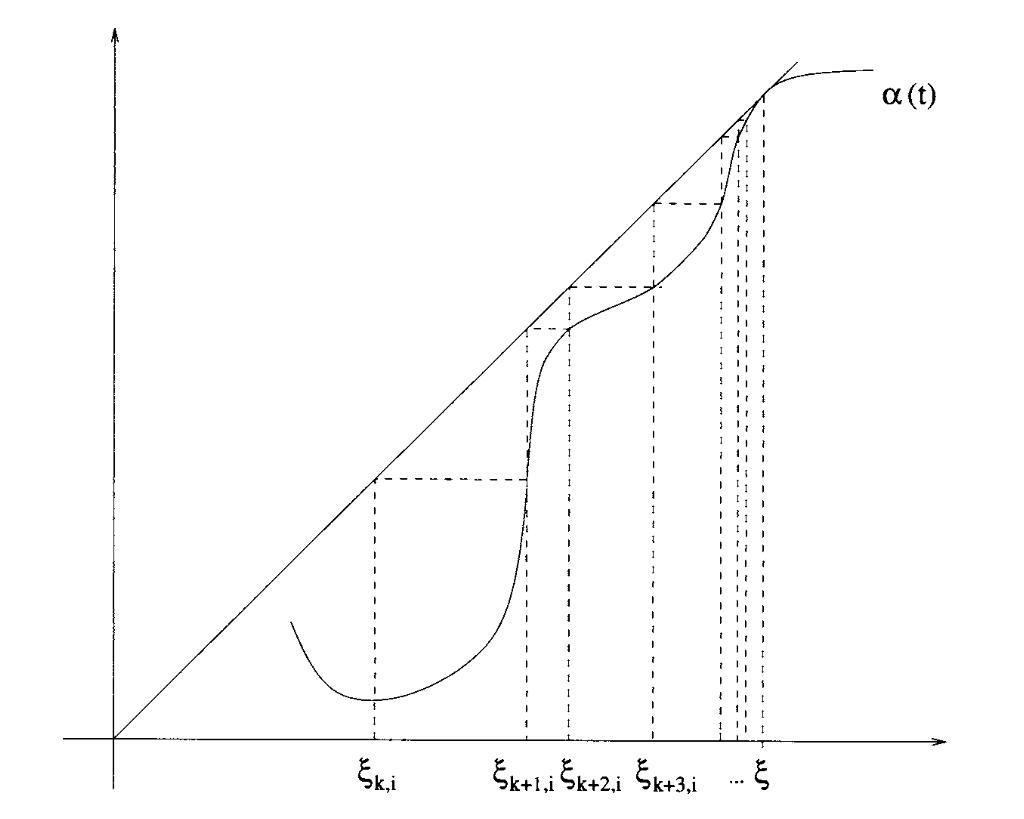
\includegraphics[width=0.9\textwidth, height=0.7\textheight]{desaparecimento_do_retardo.png}
        \end{center}
        \caption{fig:Desaparecimento do Retardo}\label{fig:Desaparecimento do Retardo}
    \end{figure}
        

\end{frame}


%%%%%%%%%%%%%%%%%%%%%%%%%%%%%%%%%%%%%%%%%%%%%%%%%%%%%%%%%%%%%%%%%%%%%%%%%%%%%%%%%%%%%%%%%%%%%%%%%%%%%%%

\begin{frame}{Retardos Limitados e Ilimitados}

    \begin{exampleblock}
        <1->{Retardos Limitados}

        $\bullet$ Caso o retardo seja limitado, a suavização da solução como visto no teorema \ref{chap2:teo:EDR_smooting}, não ocorre.


        $\bullet$ Para mostrar tanto, supoha que exista algum $M>0$ tal que \( \lim_{t \to \infty} \alpha(t) \leq M \).

        $\bullet$ Suponha que $\xi_{k, i}$ seja uma descontinuidade primária em $[M, +\infty)$, então $\alpha(t) < M < \xi_{k, j}$ para todo $t > M$, logo não existe $\xi_{k+1, i}$ que satisfaz $\alpha(\xi_{k+1, i}) = \xi_{k, j}$.
        
        $\bullet$ Segue uma ilustração deste fenômemo.

    \end{exampleblock}

\end{frame}

%%%%%%%%%%%%%%%%%%%%%%%%%%%%%%%%%%%%%%%%%%%%%%%%%%%%%%%%%%%%%%%%%%%%%%%%%%%%%%%%%%%%%%%%%%%%%%%%%%%%%%%

\begin{frame}{Retardos Limitados e Ilimitados}

    \begin{figure}
        \begin{center}
            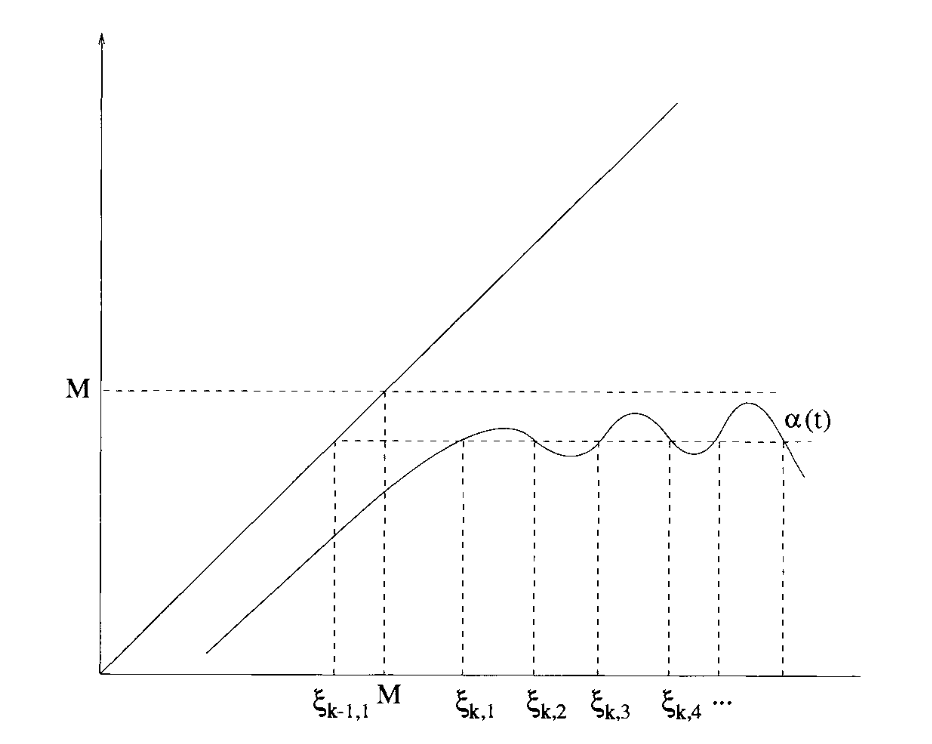
\includegraphics[width=0.9\textwidth, height=0.7\textheight]{retardo_limitado.png}
        \end{center}
        \caption{Retardo limitado}\label{fig:Desaparecimento do Retardo}
    \end{figure}

\end{frame}


%%%%%%%%%%%%%%%%%%%%%%%%%%%%%%%%%%%%%%%%%%%%%%%%%%%%%%%%%%%%%%%%%%%%%%%%%%%%%%%%%%%%%%%%%%%%%%%%%%%%%%%

\begin{frame}{Retardos Limitados e Ilimitados}
    
    $\bullet$ Para garantir a suavização das soluções, a função $\alpha$ deve setisfazer as seguintes duas hipóteses.

    \begin{hip}
        \label{H2:hipotese:hypothesis}
        $\lim _{t \rightarrow+\infty} \alpha(t)=+\infty$.
    \end{hip}


    \begin{hip}
        \label{H3:hipotese:hypothesis}
        Existe uma constante \(\tau_{1}>0\) tal que \(\tau(t)=t-\alpha(t) \leq \tau_{1}\) para todo \(t \in\left[t_{0}, t_{f}\right]\).
    \end{hip}

    $\bullet$ abaixo, segue uma figura ilustrativa dessas três hipóteses em ação.

\end{frame}



%%%%%%%%%%%%%%%%%%%%%%%%%%%%%%%%%%%%%%%%%%%%%%%%%%%%%%%%%%%%%%%%%%%%%%%%%%%%%%%%%%%%%%%%%%%%%%%%%%%%%%%

\begin{frame}{Retardos Limitados e Ilimitados}

    \begin{figure}
        \begin{center}
            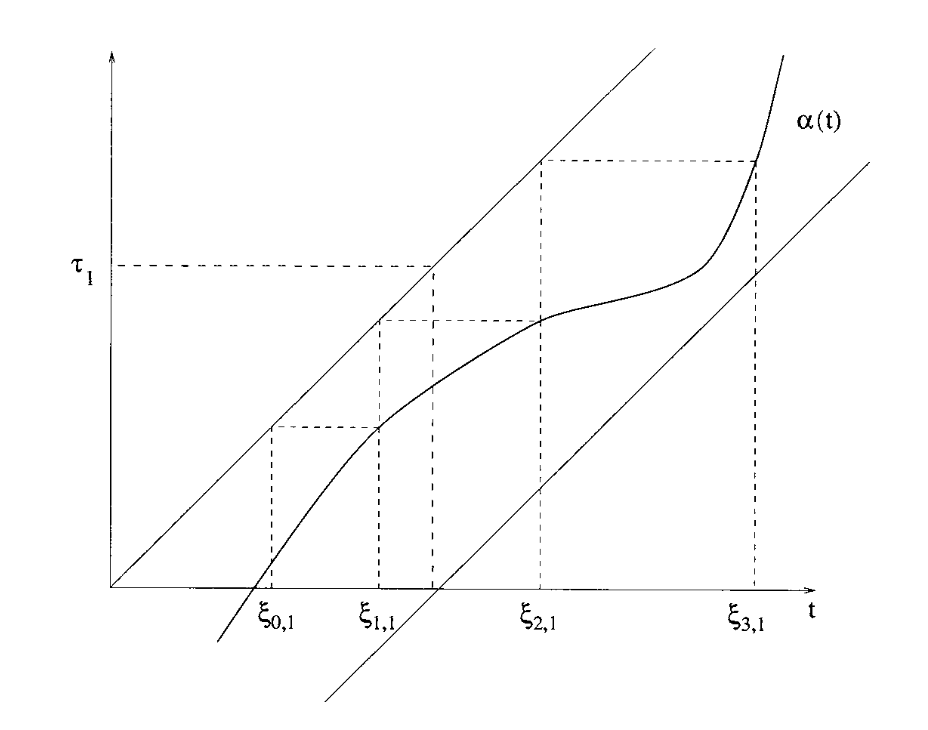
\includegraphics[width=0.9\textwidth, height=0.7\textheight]{hip123.png}
        \end{center}
        \caption{Hip 123}\label{fig:Desaparecimento do Retardo}
    \end{figure}

\end{frame}


%%%%%%%%%%%%%%%%%%%%%%%%%%%%%%%%%%%%%%%%%%%%%%%%%%%%%%%%%%%%%%%%%%%%%%%%%%%%%%%%%%%%%%%%%%%%%%%%%%%%%%%


\begin{frame}{Descontinuidades Principais}

    $\bullet$ Dentre as descontinuidades primárias, um tipo delas se destaca em importância.

    \begin{definition}
        \label{chap2:def:principal_descontinuity}
    Seja $\bar{\xi_0} = t_0$ definido como uma \textit{descontinuidade principal de nível 0}. Indutivamente, uma \textit{descontinuidade principal de nível (k+1)} é a menor raiz $\bar{\xi}_{k+1}$ de 
        \[
            \alpha(t) = \bar{\xi_k}
        \]
        com multiplicidade ímpar, sendo $\bar{\xi_k}$ uma \textit{descontinuidade principal de nível (k)}
    \end{definition}


    $\bullet$ Note que $ \alpha(t) \leq \bar{\xi}_{k}, \quad \forall t \in\left[\bar{\xi}_{k}, \bar{\xi}_{k+1}\right] $ e todo $k$

    $\bullet$ Logo, a EDR \eqref{def:eq:EDR} se reduz a uma EDO nos intervalos $\left[\bar{\xi}_{k}, \bar{\xi}_{k+1}\right]$. 

\end{frame}
%%%%%%%%%%%%%%%%%%%%%%%%%%%%%%%%%%%%%%%%%%%%%%%%%%%%%%%%%%%%%%%%%%%%%%%%%%%%%%%%%%%%%%%%%%%%%%%%%%%%%%%


\begin{frame}{Existência e unicidade de soluções}

    \small
    \begin{teo}[Existência local]
        \label{chap2:teo:local_existence:EDR}
        Teorema 2.2.4 Considere a equação \ref{chap1:def:EDRN}, ou seja,

        \[
            \left\{\begin{array}{l}
                    y^{\prime}(t)=f(t, y(t), y(t-\tau(t, y(t)))), \quad t \geq t_{0}  \\
                    y(t)=\phi(t), \quad t \leq t_{0}
            \end{array}\right.
        \]

        Sejam \(U \subseteq \mathbb{R}^{d}\) e \(V \subseteq \mathbb{R}^{d}\) vizinhanças de \(\phi\left(t_{0}\right)\) e \(\phi\left(t_{0}-\tau\left(t_{0}, \phi\left(t_{0}\right)\right)\right)\), respectivamente, e suponha que a função \(f(t, u, v)\) seja contínua em relação a \(t\) e Lipschitz contínua em relação a \(u\) e \(v\) em \(\left[t_{0}, t_{0}+h\right] \times U \times V\) para algum \(h>0\). Além disso, suponha que a função inicial \(\phi(t)\) seja Lipschitz contínua para \(t \leq t_{0}\) e que a função de atraso \(\tau(t, y) \geq 0\) seja contínua em relação a \(t\) e Lipschitz contínua em relação a \(y\) em \(\left[t_{0}, t_{0}+h\right] \times U\). Então o problema \ref{chap1:def:EDRN} tem uma única solução em \(\left[t_{0}, t_{0}+\delta\right)\) para algum \(\delta>0\) e esta solução depende continuamente dos dados iniciais.

    \end{teo}
\end{frame}

%%%%%%%%%%%%%%%%%%%%%%%%%%%%%%%%%%%%%%%%%%%%%%%%%%%%%%%%%%%%%%%%%%%%%%%%%%%%%%%%%%%%%%%%%%%%%%%%%%%%%%%

\section{Métodos Numéricos Contínuos}
\subsection{Métodos Contínuos para EDOs}

\begin{frame}{Métodos Contínuos para EDOs}
    \small
    \begin{defi}[Método de k-passos]
        Para $n = 0, ..., N-1$, sejam

        \begin{itemize}
            \item[$\bullet$] $\Delta = \{ t_0, ..., t_N = t_f\}$ uma malha,

            \item[$\bullet$] $h_{n+1} = t_{n+1} - t_n$ os passos, 
        \end{itemize}

        Um método numérico para resolver o PVI \eqref{def:eq:PVI} é chamado de \textit{método de k-passos} se ele satisfaz 

        \begin{equation}
            y_{n+1} = \alpha_{n, 1} y_n + ... + \alpha_{n, k} y_{n - k + 1} + h_{n+1} \Phi( y_n, ..., y_{n-k+1}; g, \Delta_n), 
            \label{chap3:def:eq:ODE_method}
        \end{equation}

        para $n \geq k - 1$ e para $\Delta_n = \{ t_{n - k + 1}, ..., t_n, t_{n+1}\} $.

        \begin{itemize}
            \item[$\bullet$] A função $\Phi$ é chamada de função incremento.
        \end{itemize}
        alguma função $\Phi$, chamada de função incremento e parâmetros $\alpha_{n,1},..., \alpha_{n,k}$, que definem os métodos particulares. A partir do $y_0$ dado em  \eqref{def:eq:PVI} e valores $y_1,... y_{k-1}$ iniciais, que comentaremos mais a diante como os podemos obter, a fórmula  \eqref{chap3:def:eq:ODE_method}  calcula valores $y_{n+1}$ que são aproximações para a solução exata calculada nos pontos da malha, ou seja,  $y(t_{n+1}) \approx t(t_{n+1})$.
    \end{defi}
\end{frame}

%%%%%%%%%%%%%%%%%%%%%%%%%%%%%%%%%%%%%%%%%%%%%%%%%%%%%%%%%%%%%%%%%%%%%%%%%%%%%%%%%%%%%%%%%%%%%%%%%%%%%%%

\begin{frame}{empty frame for reference}
     empty frame for reference
\end{frame}

%%%%%%%%%%%%%%%%%%%%%%%%%%%%%%%%%%%%%%%%%%%%%%%%%%%%%%%%%%%%%%%%%%%%%%%%%%%%%%%%%%%%%%%%%%%%%%%%%%%%%%%

\section{O Modelo SIR}
\subsection{Descrição Matemática}
\begin{frame}{Modelo de Kermack e McKendrick}

    \begin{exampleblock}
        <1->{Modelo SIR}
        \begin{itemize}
            \item [$\bullet$] $s,i,r :=$ Percentual de Susceptíveis, Infectados e Removidos;
            \item [$\bullet$] $\beta, \gamma := $ Taxa média de Contato e de Remoção por tempo;
            \item [$\bullet$] O modelo é dado por
                $ 
                \begin{cases}
                    \frac{ds}{dt} &= -\beta i s; \\ 
                    \frac{di}{dt} &= \beta i s - \gamma i;  \\
                    \frac{dr}{dt} &= \gamma i \gamma. 
                \end{cases}
                $ 
                onde $s + i + r = 1$;
            \item [$\bullet$] Note que a taxa de infeção é homogênea, ou seja, a chance de um indivíduo
                infectado contaminar outra pessoa é sempre a mesma, independente da pessoa. 
            \item [$\bullet$] Soluções analíticas para o modelo são difíceis de encontrar, o que não 
                nos impede de tirar conclusões importantes sobre o comportamento do modelo.

        \end{itemize}

    \end{exampleblock} 
    
\end{frame}



%%%%%%%%%%%%%%%%%%%%%%%%%%%%%%%%%%%%%%%%%%%%%%%%%%%%%%%%%%%%%%%%%%%%%%%%%%%%%%%%%%%%%%%%%%%%%%%%%%%%%%%
\subsection{Número Básico de Reprodução}
\begin{frame}{Modelo de Kermack e McKendrick}


    \begin{exampleblock}
        <1->{Número Básico de Reprodução}

        \begin{itemize}
            \item [$\bullet$] Suponha que a população sucetível seja 1. O Número Básico de Reprodução 
                $R_0$ é o número médio de pessoas que a doença é transmitida antes da pessoa ser 
                imunizada. Note que, se $R_0>1$ a doença cresce, já se $R_0<0$, a doença descresce. 
                O limiar epidemiológico é definido quando $R_0 = 1$i.
            \item [$\bullet$] No modelo SIR, a doença cresce quando $\frac{di}{dt} > 0$. Supondo que 
                $s=1$ obtemos
                \[
                 0 < \frac{di}{dt} = \beta i s - \gamma i \iff 
                 0 < \beta i - \gamma i \iff 
                 i < \frac{\beta}{\gamma}i \iff 
                 0 < \frac{\beta}{\gamma}
                \]
                ou seja, $R_0 = \frac{\beta}{\gamma}$ denota o início da epidemia.
        \end{itemize}

    \end{exampleblock} 
    
\end{frame}

%%%%%%%%%%%%%%%%%%%%%%%%%%%%%%%%%%%%%%%%%%%%%%%%%%%%%%%%%%%%%%%%%%%%%%%%%%%%%%%%%%%%%%%%%%%%%%%%%%%%%%%
\subsection{Tamanho da Epidemia}
\begin{frame}{Modelo de Kermack e McKendrick}
    \begin{exampleblock}
	     <1->{Tamanho da Epidemia}
             \begin{itemize}
                 \item [$\bullet$] O tamanho da epidemia no modelo SIR nunca é igual a $1$ 
                     independente se $R_0 >> 1$ (onde $R_0 < \infty$), ou seja 
                    \[
                        s_\infty = 1 - r_\infty > 0, \qquad \forall R_0 \in \mathbb{R}.
                    \] 
                     A demonstração deste fato é envolvida, eis um modelo visual interativo para 
                     exploração: \href{https://www.geogebra.org/classic/pbddxfeh}{geogebra}
            
\begin{center}
    
\begin{tikzpicture}[scale=0.4]
  \begin{axis}[
    xlabel={Tempo},
    ylabel={População Normalizada},
    legend style={
      at={(0.5,-0.2)},
      anchor=north,
      legend columns=3,
      draw=none,
      /tikz/every even column/.append style={column sep=0.5cm}
    },
    cycle list name=color list,
    every axis plot/.append style={line width=1.5pt},
    ]
    
    \addplot table [y expr=\thisrow{S}/1000, mark=none, col sep=comma] {data.csv};
    \addlegendentry{Suscetíveis}
    \addplot table [y expr=\thisrow{I}/1000, mark=none, col sep=comma] {data.csv};
    \addlegendentry{Infeciosos}
    
    \addplot table [y expr=\thisrow{R}/1000, mark=none, col sep=comma] {data.csv};
    \addlegendentry{Removidos}
    
    \node[align=center, anchor=north east] at (axis description cs:1,0.8) {$\beta = 0.3$ \\ $\gamma = 0.1$};
    
  \end{axis}  
\end{tikzpicture}

\end{center}                
\end{itemize}
\end{exampleblock}

\end{frame}




%%%%%%%%%%%%%%%%%%%%%%%%%%%%%%%%%%%%%%%%%%%%%%%%%%%%%%%%%%%%%%%%%%%%%%%%%%%%%%%%%%%%%%%%%%%%%

\begin{frame}{Referências}


\begin{thebibliography}{3}



\beamertemplatearticlebibitems
\bibitem{Neves1976CharacterizationOJ}
K. W. Neves and A. Feldstein,
\newblock Characterization of jump discontinuities for state dependent delay differential equations.
\newblock \emph{Journal of Mathematical Analysis and Applications},
\oldstylenums{56}:689-707,
\oldstylenums{1976}.
\newblock \url{https://api.semanticscholar.org/CorpusID:121097839}.


\beamertemplatearticlebibitems
\bibitem{neves[206]}
K. W. Neves and S. Thompson,
\newblock Software for the numerical solution of systems of functional differential equations with state-dependent delays.
\newblock \emph{Applied Numerical Mathematics},
\oldstylenums{9}(3):385-401,
\oldstylenums{1992}.
\newblock \url{https://doi.org/10.1016/0168-9274(92)90029-D}.

\end{thebibliography}
\end{frame}

%%%%%%%%%%%%%%%%%%%%%%%%%%%%%%%%%%%%%%%%%%%%%%%%%%%%%%%%%%%%%%%%%%%%%%%%%%%%%%%%%%%%%%%%%%%%%%%%


\section{Referências}
\begin{frame}{Referências}


\begin{thebibliography}{4}

\beamertemplatearticlebibitems
\bibitem{PhysRevE.66.016128}
M. E. J. Newman,
\newblock Spread of epidemic disease on networks.
\newblock\emph{Phys. Rev. E},
\oldstylenums{66}(1):016128,
\oldstylenums{2002}.

\beamertemplatearticlebibitems
\bibitem{PhysRevE.64.026118}
M. E. J. Newman, S. H. Strogatz, and D. J. Watts,
\newblock Random graphs with arbitrary degree distributions and their applications.
\newblock\emph{Phys. Rev. E},
\oldstylenums{64}(2):026118,
\oldstylenums{2001}.


\beamertemplatebookbibitems
\bibitem{Author1990}M. E. J. Newman \newblock\emph{Networks}.\newblock
\textlatin{Oxford University Press, \oldstylenums{2018}}.

\end{thebibliography}
\end{frame}



%%%%%%%%%%%%%%%%%%%%%%%%%%%%%%%%%%%%%%%%%%%%%%%%%%%%%%%%%%%%%%%%%%%%%%%%%%%%%%%%%%%%%%%%%%%%%


\end{document}

